\section{Algorithm implementation}
Next, we will implement the three chosen algorithms: MLP (Multilayer Perceptron), Autoencoder, and [Third Algorithm]. These algorithms have been selected due to their suitability for classification problems and their ability to handle structured and complex datasets. First, we will provide a brief introduction to each algorithm, highlighting their key characteristics. After that, we will proceed with the implementation and performance analysis for our dataset.

\subsection{Multilayer Perceptron (MLP)}

The \textbf{Multilayer Perceptron (MLP)} is a core model in the field of machine learning, used for both classification and regression tasks. MLP consists of three primary layers: the \textbf{input layer}, one or more \textbf{hidden layers}, and the \textbf{output layer}. Each layer contains multiple neurons, and neurons from one layer are fully connected to neurons in the next layer. This dense connectivity allows MLP to capture complex relationships in data, particularly non-linear ones, which are common in many real-world applications \cite{deeplearning1}.

In the context of our dataset, which includes health-related features such as \texttt{BMI}, \texttt{Age}, \texttt{Physical\_Health}, and \texttt{Sleep\_Time}, MLP is well-suited to identify hidden patterns and make predictions about whether an individual has diabetes or not. The network learns from the data through a process called \textit{backpropagation}, where errors from the output are propagated back through the network to adjust the weights of the connections between neurons. This process is combined with \textit{gradient descent}, an optimization technique that minimizes the prediction error by adjusting the weights during each iteration of training. Over time, the model learns the optimal weights, improving its ability to make accurate predictions \cite{nn1}.

The basic structure of an MLP is illustrated in the figure below. The input features, such as \texttt{BMI} and \texttt{Age}, are fed into the input layer. From there, they pass through one or more hidden layers, where neurons transform the data by applying learned weights and activation functions. The transformed data then flows to the output layer, which produces the final prediction, such as whether an individual has diabetes.

\begin{figure}[H]
    \centering
    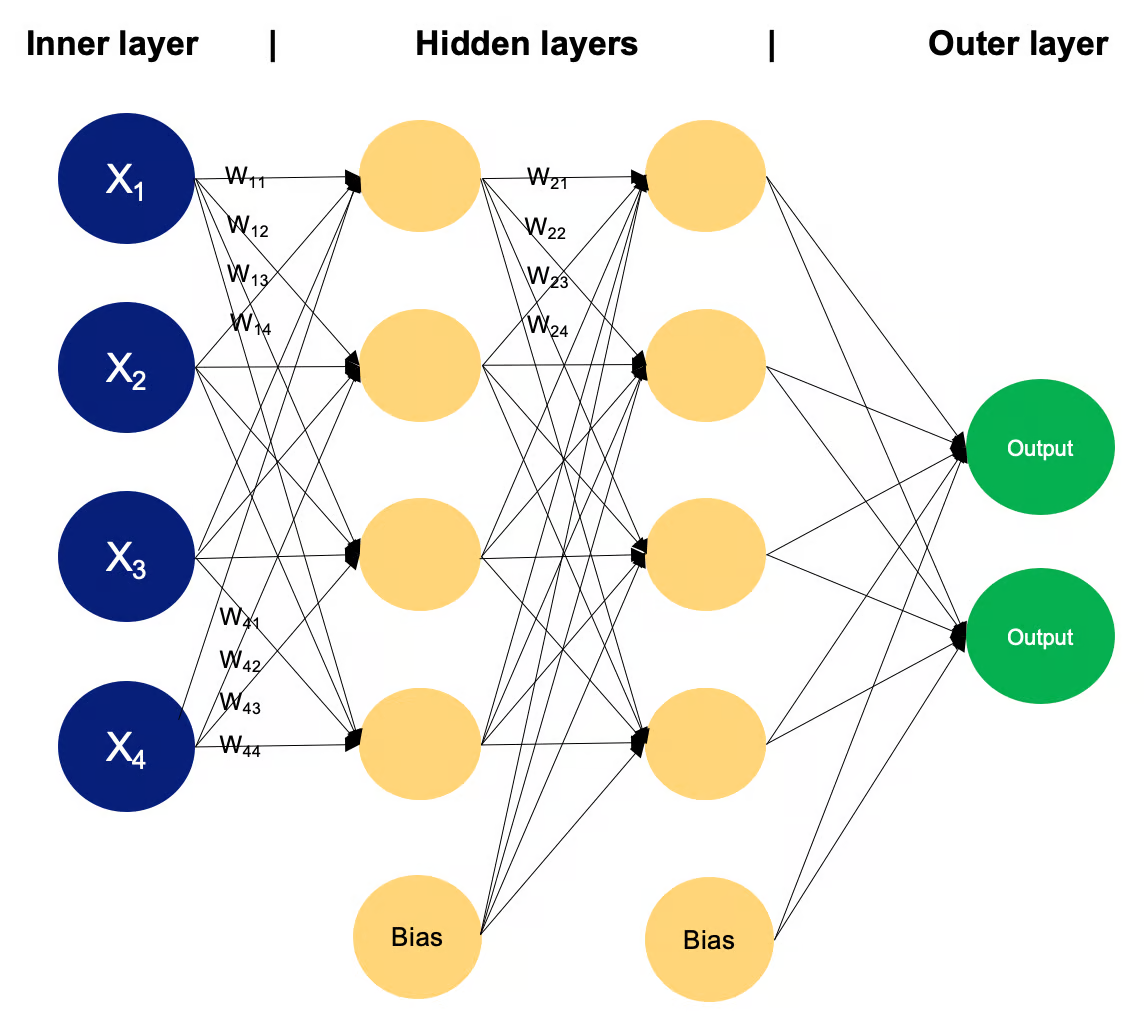
\includegraphics[width=0.7\textwidth]{images/mlp-diagram.png}
    \caption{Basic structure of a Multilayer Perceptron (MLP) \cite{mlp}.}
    \label{fig:mlp}
\end{figure}

In the image, you can observe the flow of information from the input layer through the hidden layers to the output layer. Each layer plays a critical role in transforming the input data to make sense of the patterns and relationships. The neurons in the hidden layers learn features in the data, and as the network adjusts its weights through training, it becomes more accurate in predicting the target outcome.

MLPs are particularly effective in tasks where the relationships between input features and the target variable are non-linear, as is the case in health-related predictions like diabetes classification \cite{deeplearning1}. This model's ability to learn from complex and large datasets allows it to handle a wide variety of problems, from image recognition to medical diagnoses.

What makes MLPs particularly well-suited for our dataset is their capacity to model intricate relationships between multiple features simultaneously. By learning these relationships, MLPs can make accurate predictions, even when the data contains complex, interdependent factors. This makes MLP an ideal choice for predicting the likelihood of diabetes based on a variety of health indicators \cite{mlp}.

\subsubsection{Implementation and Evaluation}

The MLP model was implemented using the \texttt{scikit-learn} library, leveraging two hidden layers with sizes 100 and 50 respectively. The activation function used was ReLU, and stochastic gradient descent was chosen as the optimizer with adaptive learning rate and a maximum of 500 iterations.

Before finalizing the model, we performed hyperparameter tuning using GridSearchCV to identify the best combination of parameters. This ensures that the model generalizes well to unseen data.

\noindent
The best parameters found were:
\begin{quote}
\texttt{\{'mlp\_\_activation': 'relu', 'mlp\_\_alpha': 0.001, 'mlp\_\_hidden\_layer\_sizes': (100, 50), 'mlp\_\_learning\_rate': 'adaptive', 'mlp\_\_max\_iter': 500, 'mlp\_\_solver': 'sgd'\}}
\end{quote}

\lstinputlisting[language=python]{../code/mlp.py}

\begin{figure}[H]
    \centering
    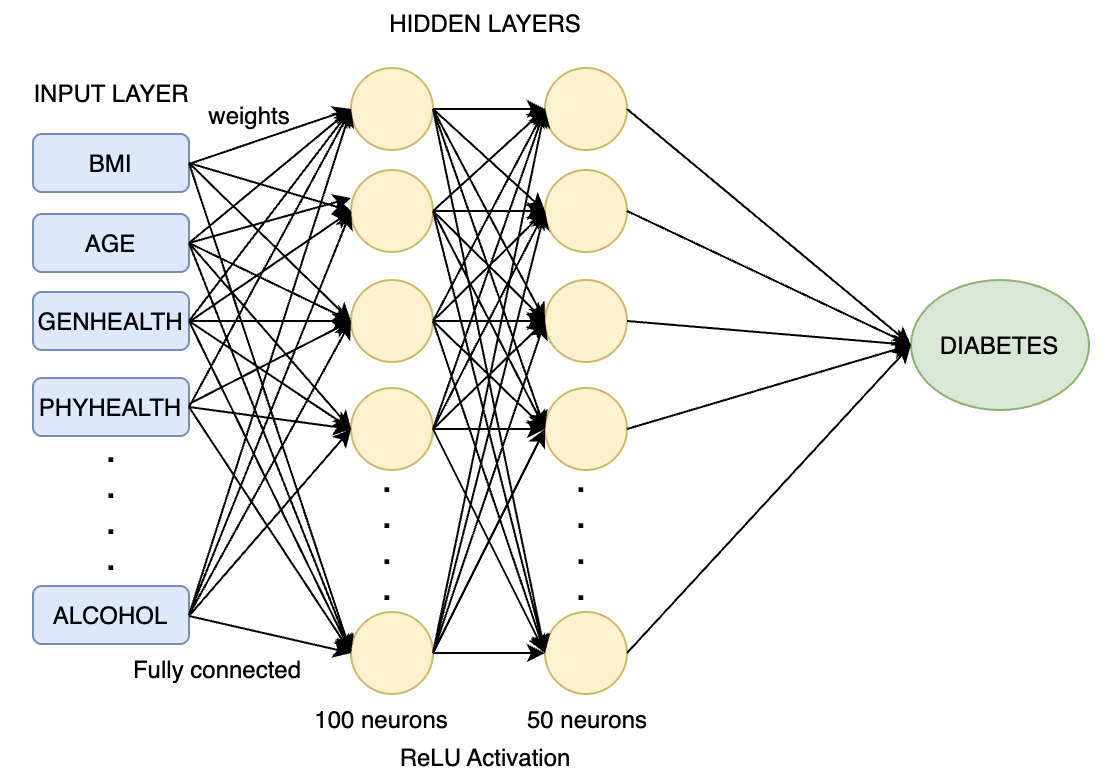
\includegraphics[width=0.75\textwidth]{images/our-mlp-diagram.png} % Make sure the filename matches
    \caption{Our structure of a Multilayer Perceptron (MLP).}
    \label{fig:mlp-arch}
\end{figure}

\vspace{0.5em}

\noindent
Figure~\ref{fig:mlp-arch} illustrates the architecture of the Multilayer Perceptron used in our implementation. It includes an input layer that receives features such as \texttt{BMI}, \texttt{Age}, and \texttt{GenHealth}, followed by two hidden layers with 100 and 50 neurons respectively. These layers apply ReLU activation and are fully connected. The final layer outputs a binary prediction indicating whether the individual is diabetic or not.


\subsubsection{Results on Full Feature Set}

\begin{verbatim}
Performance on Full Feature Set:
Accuracy: 0.7526
Precision: 0.7362
Recall: 0.8011
F1 Score: 0.7673
\end{verbatim}

\noindent
This baseline performance shows that the MLP model handles the full feature set well, achieving over 75\% accuracy and strong recall (80.11\%). Precision and F1-score are also relatively balanced, which means the model is both identifying and distinguishing cases effectively.

\vspace{0.5em}
\noindent
Next, we look at cross-validation results to assess the model’s ability to generalize across different data splits:

\begin{verbatim}
Cross-Validation Mean Scores (5-Fold):
Accuracy: Train = 0.7558, Test = 0.7484
Precision: Train = 0.7359, Test = 0.7295
Recall: Train = 0.8113, Test = 0.8040
F1: Train = 0.7718, Test = 0.7649
\end{verbatim}

\noindent
These results confirm that the model generalizes well, as train and test scores remain consistent across folds. Importantly, test recall remains high (80.40\%), reinforcing the model’s reliability in correctly identifying diabetic cases in unseen data. This cross-validation step validates the single-run results and supports the model’s robustness.

\vspace{0.5em}
\noindent
Now we present the full classification report to explore class-wise performance in more detail:

\begin{verbatim}
Detailed Classification Report (Full Feature Set):
              precision    recall  f1-score   support

 No Diabetes       0.77      0.70      0.74      6753
    Diabetes       0.74      0.80      0.77      7000

    accuracy                           0.75     13753
   macro avg       0.75      0.75      0.75     13753
weighted avg       0.75      0.75      0.75     13753
\end{verbatim}

\begin{figure}[H]
    \centering
    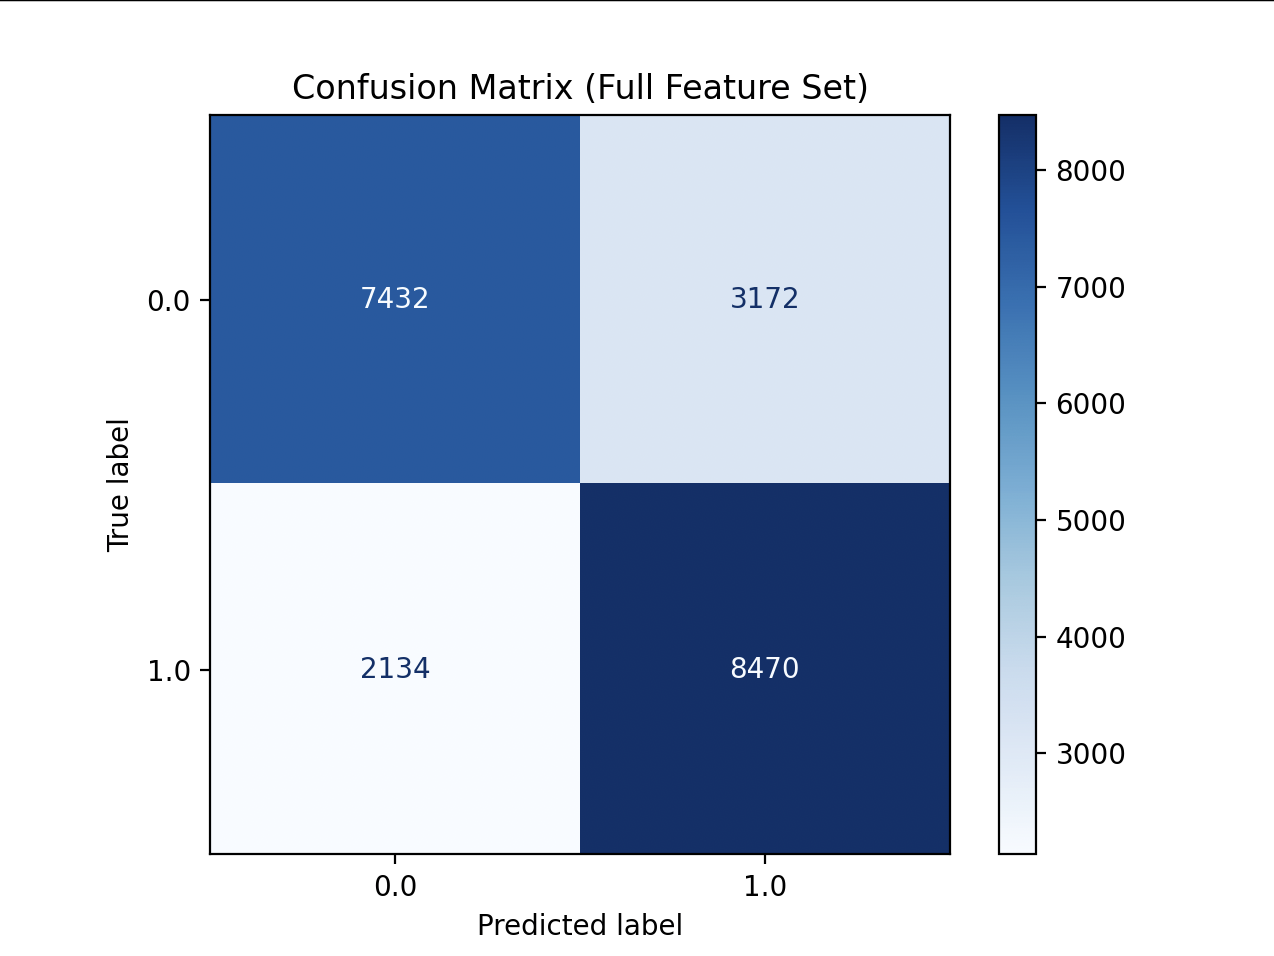
\includegraphics[width=0.5\textwidth]{images/confusion_matrix_full.png}
    \caption{Confusion Matrix for MLP on Full Feature Set}
\end{figure}

\noindent
From this report, it's evident that the model performs slightly better at detecting positive (diabetic) cases than negative ones, with a higher recall for the "Diabetes" class (80\%). This is desirable in our context: it is far more critical to minimize false negatives (undiagnosed diabetic patients) than false positives. Therefore, recall is the metric we prioritize most.

\subsubsection{Results on Selected Features with Interaction Terms}

\begin{verbatim}
Performance on Selected Features + Interactions:
Accuracy: 0.6917
Precision: 0.6633
Recall: 0.8007
F1 Score: 0.7256
\end{verbatim}

\noindent
While accuracy and precision have dropped in this simplified model, recall has remained nearly identical (80.07\%) to the full-feature model. This suggests that the reduced feature set is still effective in identifying diabetic patients, even if it leads to more false positives (lower precision).

\vspace{0.5em}
\noindent
We now show the detailed classification report for this model:

\begin{verbatim}
Detailed Classification Report (Interactions Model):
              precision    recall  f1-score   support

 No Diabetes       0.74      0.58      0.65      6753
    Diabetes       0.66      0.80      0.73      7000

    accuracy                           0.69     13753
   macro avg       0.70      0.69      0.69     13753
weighted avg       0.70      0.69      0.69     13753
\end{verbatim}

\begin{figure}[H]
    \centering
    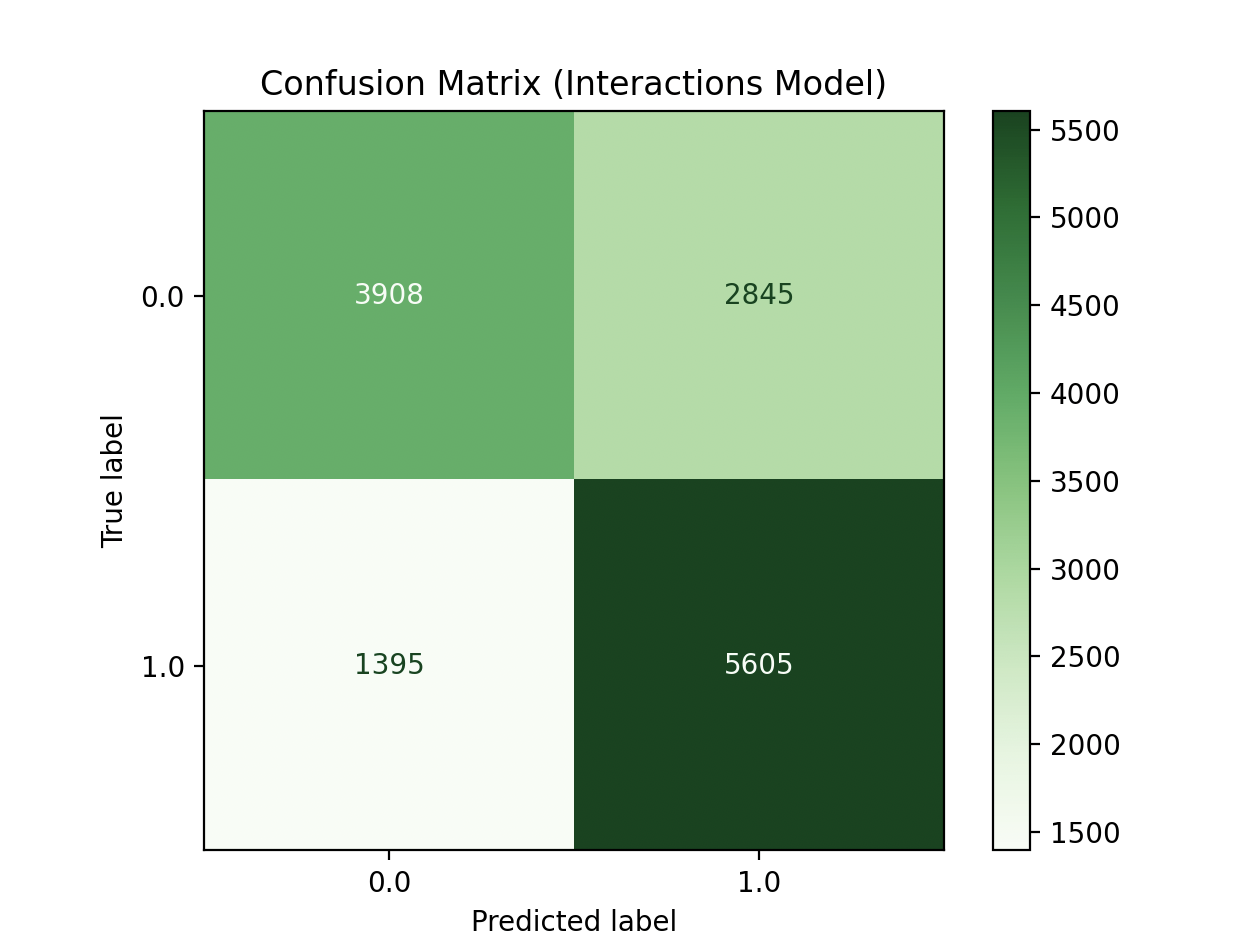
\includegraphics[width=0.5\textwidth]{images/confusion_matrix_interactions.png}
    \caption{Confusion Matrix for MLP on Selected Features + Interaction Terms}
\end{figure}

\noindent
Here again, recall for diabetic cases remains at 80\%, but performance for non-diabetic predictions drops noticeably (recall of 58\%). In practice, this means more people without diabetes are misclassified as diabetic. While this may raise false alarms, it is an acceptable trade-off in medical diagnostics where missing true cases is more dangerous than flagging potential ones.

\vspace{1em}
\noindent
In both models, recall is prioritized above all, aligning with our goal of reducing undiagnosed diabetic cases. The full-feature model is preferred for balanced performance, but the interaction-based model still holds value in more constrained environments.

\begin{figure}[H]
    \centering
    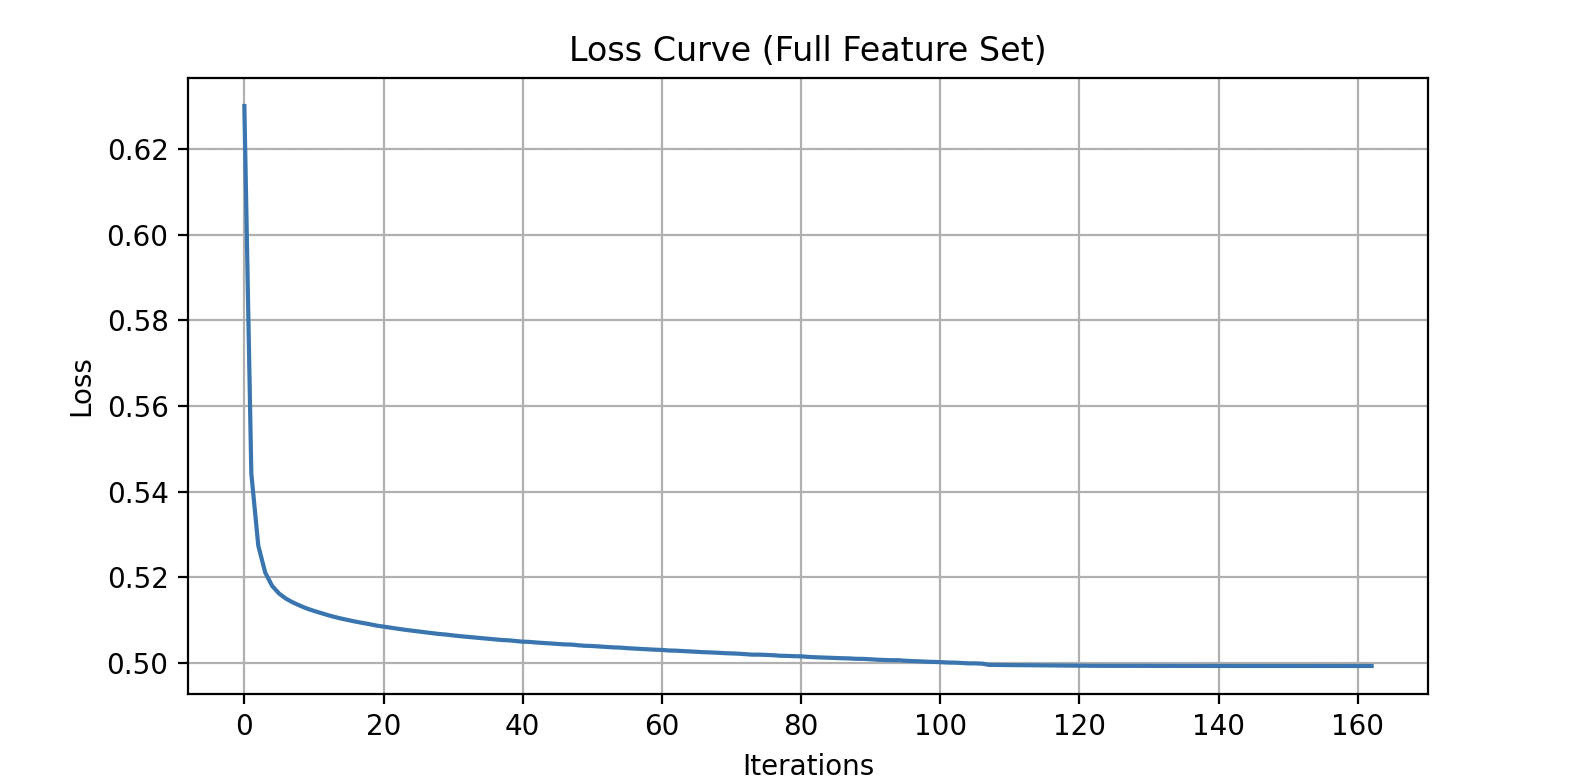
\includegraphics[width=0.6\textwidth]{images/mlp-loss-curve.png} 
    \caption{Training loss curve for the MLP model over 500 iterations.}
    \label{fig:mlp_loss_curve}
    \end{figure}

The loss curve for the diabetes dataset shows a rapid initial decrease followed by convergence, indicating stable training and successful optimization.


\subsection{Autoencoder}

\subsection{Third algorithm}